\chapter{Introduction}
\label{cha:Introduction}

The terms 'autonomous vehicle' and 'self-driving car' were once thought of as science fiction, but as of recent, they have become our reality. Google's Self-Driving Car Project is gaining traction, with cars currently driving \newtext{in Milton Keynes and }four different US states \citep{GoogleCars}. Tesla Motors have deployed a beta version of their Autopilot system into all of their vehicles produced since September 2014. The system has been blamed for both saving and ending lives \citep{TeslaHospital} \citep{TeslaUnderInvestigation}. 2016 has been a big year for autonomous vehicles and with that comes an even bigger push for robust and secure autonomous systems.
The possible benefits of autonomous vehicles cover a lot of different areas of concern. 

The main issue it addresses is safety. Autonomous vehicles would be able to react to incidents on the road much more quickly than a human driver would. A human's 'thinking distance' can often determine whether someone survives an accident or not. This distance can also be greatly increased if the driver of the vehicles is under the influence of alcohol or narcotics. An autonomous vehicle however, would be able to react to accidents much more quickly than a human, reducing the thinking distance greatly, improving road safety.

\begin{figure}[h]
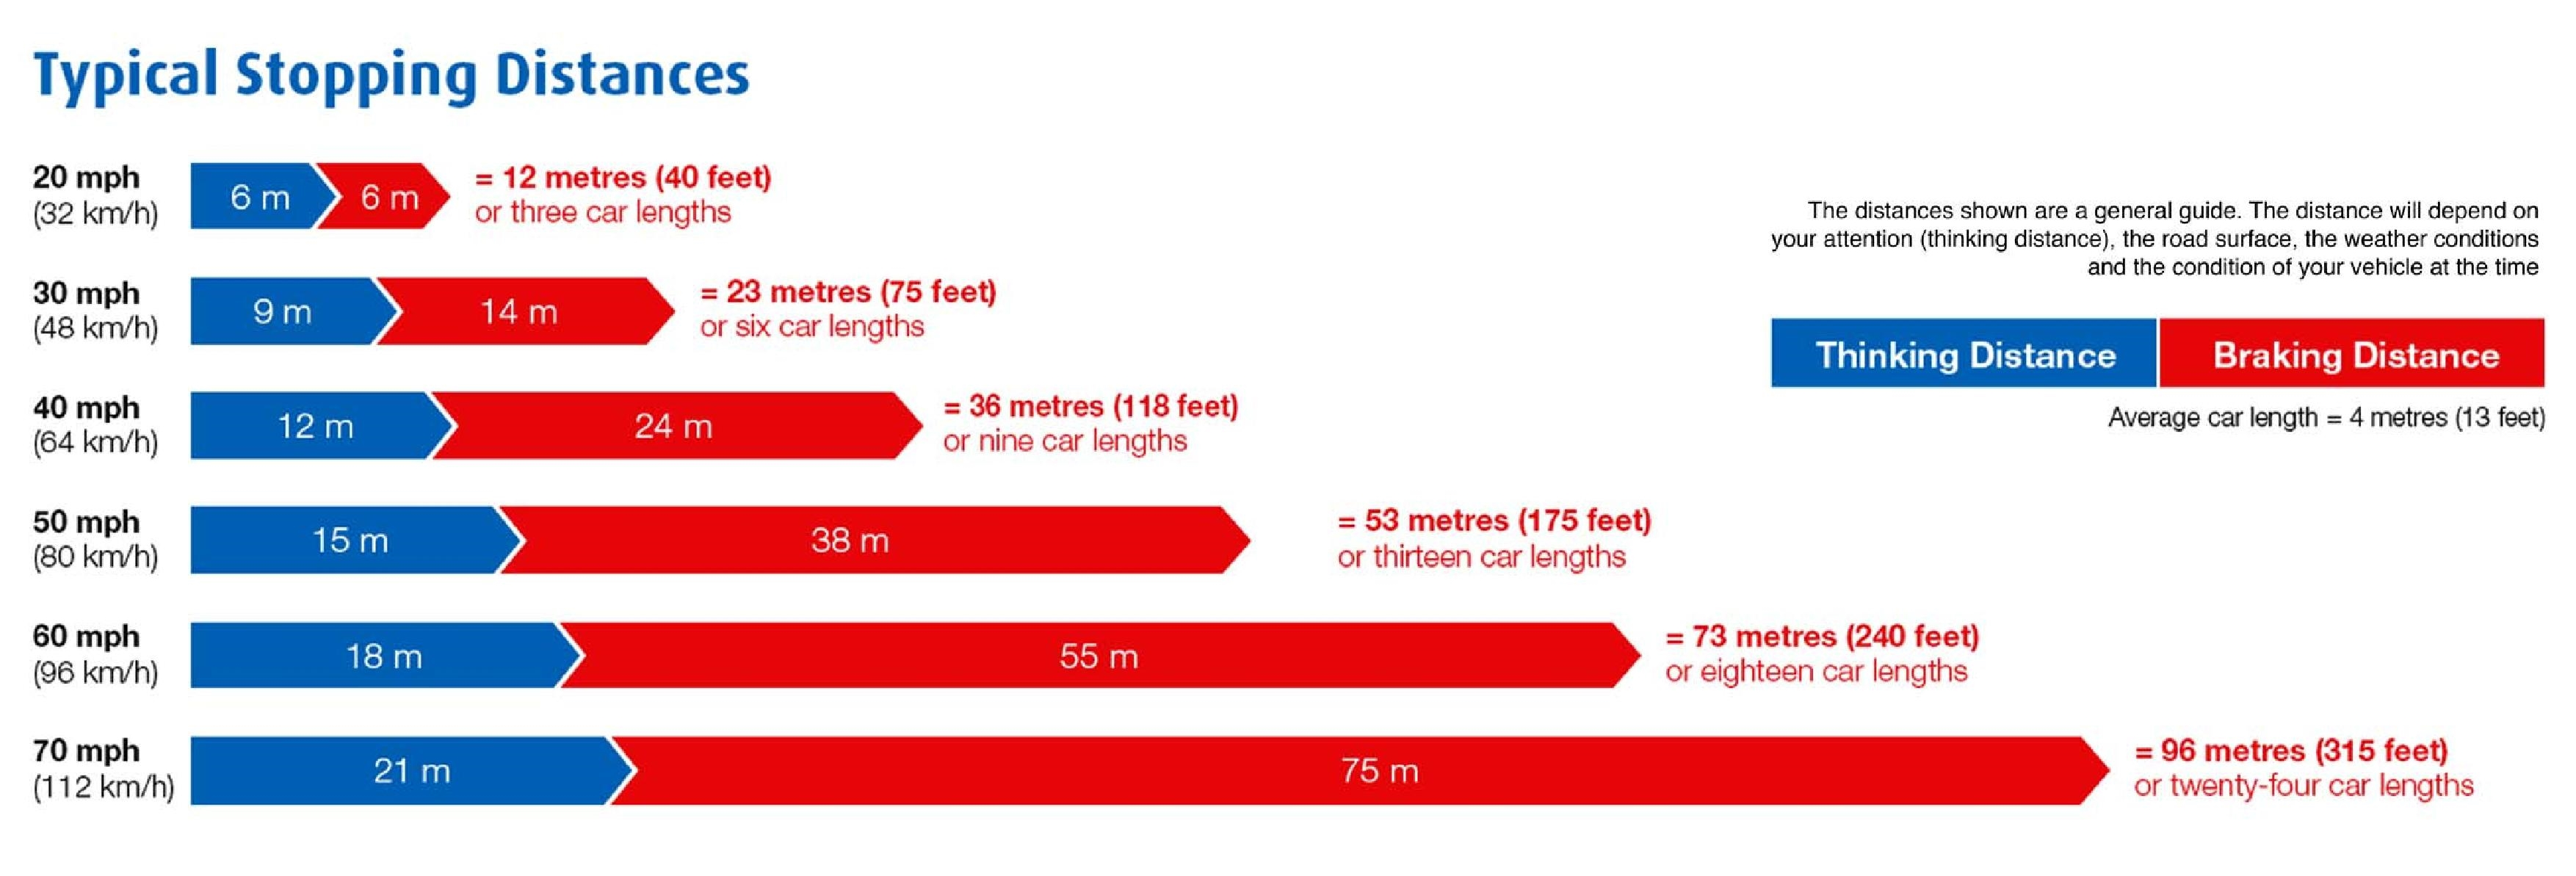
\includegraphics[width=\textwidth]{stoppingDistances.jpg}
\caption{Diagram from Rule 126 in the UK Highway Code \citep{StoppingDistances}}
\end{figure}

Autonomous vehicles could also make transport more efficient. Research by Mersky in April 2016 suggested that fuel conservation control strategies could make autonomous vehicles up to 10\% more fuel efficient than current EPA fuel economy test results \citep{Mersky2016} \todo{Read this article}. Having vehicles which are fuel efficient is becoming increasingly important, with landmark climate change deals such as 'The Paris Agreement' introducing limits on greenhouse gas emissions globally. The introduction of electric vehicles into the car market is also an important factor to consider, as the range of such vehicles still has not managed to match that of their gasoline counterparts. More efficient driving strategies introduced by autonomous vehicles could reduce this gap.

\newtext{Congestion contributes to fuel loss in quite a large way. In the US in 2014 an estimated 3.1 billion gallons (11.7 billion litres) of fuel was wasted due to congestion \citep{Schrank2015}. Automating typical driving activities and communications between vehicles, in situations such as lane changes, could reduce congestion and improve efficiency. Unsafe lane changes don't even have to result in a crash to cause delays. If a car brakes due to a car merging unsafely it can cause a ripple effect, creating a traffic jam.}

Autonomous vehicles also offer a level of comfort not currently available today. In a world where autonomous vehicles are commonplace, it is not hard to imagine people doing work, reading or relaxing in their car instead of having to focus on driving. 

However, today there are still a number of concerns surrounding autonomous vehicles. One of the major concerns is over the reliability of the systems governing the vehicle. These systems need to be responsive and accurate and they cannot afford to fail in such safety critical environments. Already concerns over Tesla's Autopilot system are impacting the image of the company, and the system isn't even out of beta testing yet \citep{TeslaCriticised}. 

In order to address these concerns safely, we can create simulations which test our autonomous systems. These simulations can test the reliability of our systems. Researchers at the University of Texas set up the Autonomous Intersection Management (AIM) project, which aims to " create a scalable, safe, and efficient multiagent framework for managing autonomous vehicles at intersections" \citep{AIMProject}. The project managed to apply their tested intersection software in a mixed reality test using a real life autonomous vehicle \citep{Quinlan2010}, demonstrating how simulations are vital tools when testing these safety critical systems.

\newtext{In this project we make a number of assumptions. Firstly we assume that the sensors resolving the positions of the vehicle and it's surrounding obstacles are perfectly accurate. We also assume that the vehicle can communicate reliably with other vehicles. These assumptions are existing areas of research for autonomous vehicles but are not considered in this paper. The main focus here is on how autonomous vehicles can self-organise to minimise delays in traffic with effective, safe lane merging.}

The aims of this project are as follows:
\begin{itemize}
\item Attempt to generalise the AIM codebase such that other simulations can be created for non-intersection related situations.
\begin{itemize}
\item If the codebase proves difficult to refactor, new simulator code will need to be created
\end{itemize}
\item Use the new codebase to create a decentralised system for managing lane merging.
\item Use the new codebase to create a centralised system for managing lane merging.
\item Compare the effectiveness of both strategies.
\end{itemize}

Creating these simulations helps to determine the effectiveness of two different strategies and also provides a codebase within which future simulations for other situations can be created.